% Graphic for TeX using PGF
% Title: /home/linfan/work/paper/myJCP/pictures/Diagram1.dia
% Creator: Dia v0.97.3
% CreationDate: Fri Feb 22 15:38:20 2019
% For: linfan
% \usepackage{tikz}
% The following commands are not supported in PSTricks at present
% We define them conditionally, so when they are implemented,
% this pgf file will use them.
\documentclass{standalone}
\usepackage{tikz}
\usepackage{amsmath,bm}

\ifx\du\undefined
  \newlength{\du}
\fi
\setlength{\du}{15\unitlength}
\begin{document}

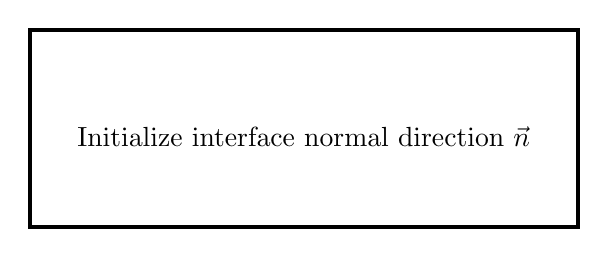
\begin{tikzpicture}
\pgftransformxscale{1.000000}
\pgftransformyscale{-1.000000}
\definecolor{dialinecolor}{rgb}{0.000000, 0.000000, 0.000000}
\pgfsetstrokecolor{dialinecolor}
\definecolor{dialinecolor}{rgb}{1.000000, 1.000000, 1.000000}
\pgfsetfillcolor{dialinecolor}
\definecolor{dialinecolor}{rgb}{1.000000, 1.000000, 1.000000}
\pgfsetfillcolor{dialinecolor}
\fill (20.950000\du,6.400000\du)--(20.950000\du,11.150000\du)--(34.150000\du,11.150000\du)--(34.150000\du,6.400000\du)--cycle;
\pgfsetlinewidth{0.100000\du}
\pgfsetdash{}{0pt}
\pgfsetdash{}{0pt}
\pgfsetmiterjoin
\definecolor{dialinecolor}{rgb}{0.000000, 0.000000, 0.000000}
\pgfsetstrokecolor{dialinecolor}
\draw (20.950000\du,6.400000\du)--(20.950000\du,11.150000\du)--(34.150000\du,11.150000\du)--(34.150000\du,6.400000\du)--cycle;
% setfont left to latex
\definecolor{dialinecolor}{rgb}{0.000000, 0.000000, 0.000000}
\pgfsetstrokecolor{dialinecolor}
\node at (27.550000\du,8.970000\du){Initialize interface normal direction $\vec{n}$};
% setfont left to latex
\definecolor{dialinecolor}{rgb}{0.000000, 0.000000, 0.000000}
\pgfsetstrokecolor{dialinecolor}
\node[anchor=west] at (27.550000\du,8.775000\du){};
\end{tikzpicture}
\end{document}